\documentclass[letterpaper, 12pt]{article}
\usepackage{geometry}
\geometry{
    letterpaper,
    left=20mm,
    top=20mm,
    bottom=20mm
}
\usepackage{tocloft}
\usepackage{graphicx}
\usepackage{authblk}
\usepackage{amssymb}
\usepackage{lipsum}
\usepackage{float}
\usepackage{times}
\usepackage{amsmath}
\usepackage[format=plain,
            labelfont={bf,it},
            textfont=it]{caption}
\captionsetup{justification=raggedright,singlelinecheck=false}
\usepackage{ragged2e}
\usepackage{longtable}
\usepackage{comment}
\usepackage{setspace}
\usepackage{fancyhdr}
\usepackage{titlesec}
\usepackage[hyperindex,breaklinks]{hyperref}
\hypersetup{
    colorlinks=true,
    linkcolor=blue,
    filecolor=magenta,      
    urlcolor=blue
}
\usepackage[T1]{fontenc}
\usepackage{helvet}
\renewcommand{\familydefault}{\sfdefault}
\pagenumbering{gobble}
\usepackage[skip=10pt plus1pt, indent=40pt]{parskip}
\usepackage{orcidlink}
\usepackage{standalone}

\titlespacing*{\section}
{0pt}{1.5ex plus 1ex minus .2ex}{1.3ex plus .2ex}

\renewcommand\Authfont{\fontsize{12}{14.4}\selectfont}
\renewcommand\Affilfont{\fontsize{9}{10.8}\itshape}

\newcommand{\cosigpart}[1]{
  \addcontentsline{toc}{part}{#1}
}
\newcommand{\cosigsection}[1]{
  \section*{#1}
  \phantomsection % avoid warnings from hyperref about the anchor of a bookmark and its parent's
  \addcontentsline{toc}{section}{#1}
}
\begin{document}
\flushleft
\includegraphics[width=0.5\textwidth]{img/home/241017_final_logo_mockup.png}

\cosigsection{Evaluating the performance of multiclass classifiers}
\textit{Last updated: 22 May 2025}

A \href{https://en.wikipedia.org/wiki/Classification_rule}{classifier} is a procedure that sorts objects in a population into classes. Multiclass classification is a classification task where there are more than two possible classes (e.g., the classification of citrus fruit as either lemon, orange or tangerine). Evaluation of multiclass classifiers is similar in many ways to the evaluation of binary classifiers (see COSIG's \href{https://osf.io/pvr4a}{entry on binary classifiers here}).

The most common method for evaluating multiclass classifiers involves treating each class as its own binary classification problem, calculating class-wise metrics like precision/positive predictive value, recall/sensitivity and F1 score (described in greater detail in COSIG's \href{https://osf.io/pvr4a}{entry on binary classifiers}) and then reporting averages of these metrics across metrics. For example, consider the following confusion matrix/contingency table:

\begin{center}
\begin{tabular}{l|ccc}
& \multicolumn{3}{c}{predicted class} \\
true class & lemon & orange & tangerine \\
\hline
lemon & 1 & 1 & 0\\
orange & 0 & 1 & 2\\
tangerine & 0 & 0 & 1\\
\end{tabular}
\end{center}

There are three objects that belong to the true class `orange'. Thus, orange has a \emph{support} of 3. When evaluating the class-wise metrics for orange, these three objects would be described as positives (P). Any objects that have the true class of `orange' and a predicted class of `orange' are described as true positives (TP). There is one such object in this confusion matrix. Any objects that have the predicted class `orange' but belong to a true class other than `orange' are described as false positives (FP). There is one such object in this confusion matrix, an instance where a lemon was incorrectly classified as an orange. Among all objects that are predicted to be oranges, one is actually an orange and one is not actually an orange. Thus, the precision for oranges is TP/(TP + FP) = 1/(1+1) = 0.5. Among all actual oranges, one is predicted to be an orange and two are predicted to not be oranges. Thus, the recall for oranges is TP/P = 1/(1+2) = 0.33. The F1 score for oranges is would then be the \href{https://en.wikipedia.org/wiki/Harmonic_mean}{harmonic mean} of its precision and recall: 0.4.

These metrics would then be calculated for each class and averaged across them. The \emph{macro average} would be the simple \href{https://en.wikipedia.org/wiki/Arithmetic_mean}{arithmetric mean} of each metric across all classes. In this example, lemon has a precision of 1.0, orange has a precision of 0.5 and tangerine has a precision of 0.33, so the macro average of precision would be (1.0 + 0.5 + 0.33)/3 = 0.611. The \emph{weighted average} of each metric would be the arithmetic mean of the metric weighted by the support of each class. In this example, lemon has a precision of 1.0 and a support of 2, orange has a precision of 0.5 and a support of 3 and tangerine has a precision of 0.33 and a support of 1, so the weighted average of precision would be (1.0 $\cdot$ 2 + 0.5 $\cdot$ 3 + 0.33 $\cdot$ 1)/6 = 0.639.

Calculation of \emph{accuracy} remains the same as with binary classification---it is the proportion of all objects that were predicted correctly. In this example, three out of six objects were predicted correctly, so accuracy is 3/6 = 0.5. Accuracy will always be greater than or equal to 0.0 and less than or equal to 1.0.

The metrics are often presented a table, often in the same style as that which is returned by the \verb|classification_report| \href{https://scikit-learn.org/stable/modules/generated/sklearn.metrics.classification_report.html}{function} of the popular \href{https://scikit-learn.org/stable/index.html}{Python package} \verb|scikit-learn|. The output of this function for the example contingency table is shown below.
\begin{center}
\begin{verbatim}
              precision    recall  f1-score   support

       lemon       1.00      0.50      0.67         2
      orange       0.50      0.33      0.40         3
   tangerine       0.33      1.00      0.50         1

    accuracy                           0.50         6
   macro avg       0.61      0.61      0.52         6
weighted avg       0.64      0.50      0.51         6
\end{verbatim}
\end{center}

\pagebreak

\subsection*{Example 1: Nonsensical confusion matrix}

\href{https://doi.org/10.1155/2022/6451199}{Wang and Yao (2022)} report on using a neural network to predict emotions from facial expressions. In Figure 3 they present a confusion matrix in which the values are not integers (and thus do not represent counts) but also do not sum to 1.0/100\% on columns nor rows (and thus do not represent proportions).

\begin{figure}[h!tbp]
    \centering
    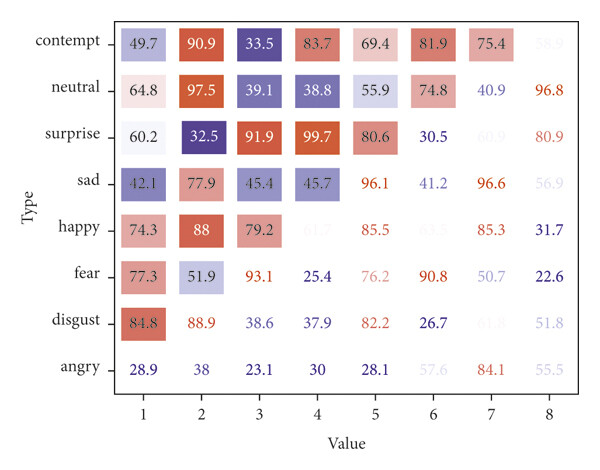
\includegraphics[width=0.8\textwidth]{img/multiclass_classifiers/wang_and_yao_fig_3.jpg}
    \caption*{Adapted from Figure 3 of \href{https://doi.org/10.1155/2022/6451199}{Wang and Yao (2022)}.}
\end{figure}

\pagebreak

\subsection*{Example 2: Impossible accuracy, F1, precision and recall scores}

\href{https://doi.org/10.1109/IC3I59117.2023.10397896}{Sharma et al. (2023)} report on models for predicting disease. At many points throughout the text, the authors report values for evaluation metrics that are not possible, such as when they claim that a model ``excels with an f1
score of 0.11 and an accuracy of 1.76'' (accuracy cannot be greater than 1.0). Table 2 reports the results for a classifier designed to assign heartbeat rhythms one of five classes. Several values for precision, recall, F1 score and the averages thereof are greater than 1.0, also impossible. Further, the support values for each class sum to 21,500, greater than the support of 12,781 reported for the macro and weighted averages. An \href{https://doi.org/10.1109/IC3I59117.2023.10703725}{expression of concern} was issued for this article in 2024.

\bgroup
\def\arraystretch{1.3}
\begin{table}[h!tbp]
\centering
\small
\begin{tabular}{|l|l|l|l|l|}
\hline
\textbf{Class} & \textbf{Precision} & \textbf{Recall} & \textbf{F1-Score} & \textbf{Support} \\ \hline
Normal Beat                       & 1.87 & 1.99 & 0.99 & 09,007 \\ \hline
Supraventricular premature beat   & 1.81 & 1.67 & 0.83 & 445    \\ \hline
Premature ventricular contraction & 1.76 & 1.84 & 0.95 & 9337   \\ \hline
Fusion of ventricular             & 1.77 & 1.41 & 0.64 & 254    \\ \hline
Unclassifiable beat               & 1.88 & 1.88 & 0.99 & 2457   \\ \hline
accuracy                          &      &      & 1.76 & 12,771 \\ \hline
macro avg                         & 1.83 & 0.84 & 1.77 & 12,781 \\ \hline
weighted avg                      & 1.87 & 0.98 & 1.87 & 12781  \\ \hline
\end{tabular}
\caption*{Adapted from Table 2 of \href{https://doi.org/10.1109/IC3I59117.2023.10397896}{Sharma et al. (2023)}.}
\end{table}
\egroup

\subsection*{Additional resources}

\begin{itemize}
    \setlength\itemsep{-0.5em}
    \item \href{https://doi.org/10.1016/j.aci.2018.08.003}{``Classification assessment methods'' (2020)}
    \item  \href{https://osf.io/pvr4a}{COSIG: Evaluating the performance of binary classifiers}
\end{itemize}

\end{document}